\documentclass[aspectratio=169]{beamer}
\usepackage[utf8]{inputenc}
\usepackage{fontspec}
\setmainfont{Times New Roman}
\setsansfont{Arial}
\usepackage{graphicx}
\usepackage{booktabs}
\usepackage{hyperref}
\usepackage{amsmath}
\usepackage{listings}
\usepackage{xcolor}

% Define colors for code listings
\definecolor{codegreen}{rgb}{0,0.6,0}
\definecolor{codegray}{rgb}{0.5,0.5,0.5}
\definecolor{codepurple}{rgb}{0.58,0,0.82}
\definecolor{backcolour}{rgb}{0.95,0.95,0.92}

\lstdefinestyle{mystyle}{
    backgroundcolor=\color{backcolour},   
    commentstyle=\color{codegreen},
    keywordstyle=\color{magenta},
    numberstyle=\tiny\color{codegray},
    stringstyle=\color{codepurple},
    basicstyle=\ttfamily\footnotesize,
    breakatwhitespace=false,         
    breaklines=true,                 
    captionpos=b,                    
    keepspaces=true,                 
    numbers=left,                    
    numbersep=5pt,                  
    showspaces=false,                
    showstringspaces=false,
    showtabs=false,                  
    tabsize=2
}
\lstset{style=mystyle}

\usetheme{Madrid}

\title[Chương 8: Giảm chiều dữ liệu]{Học Máy (Machine Learning)\\Chương 8: Giảm chiều dữ liệu (Dimensionality Reduction)}
\author{Giảng viên: TS. Trần Thành Thắng}
\institute{Đại học Đông Á}
\date{\today}

\begin{document}

% Slide 1
\begin{frame}
    \titlepage
\end{frame}

% Slide 2
\begin{frame}{Nội dung Chương trình}
    \tableofcontents
\end{frame}

\section{Khái quát về Giảm chiều dữ liệu}
% Slide 3
\begin{frame}{Giới thiệu Giảm chiều dữ liệu}
    \begin{itemize}
        \item Trong thực tế, nhiều bài toán học máy liên quan đến hàng nghìn hoặc hàng triệu đặc trưng (features) cho mỗi trường hợp huấn luyện.
        \item Việc này không chỉ làm quá trình huấn luyện cực kỳ chậm mà còn làm cho việc tìm ra một giải pháp tốt trở nên khó khăn hơn.
        \item Vấn đề này thường được gọi là \textbf{lời nguyền của số chiều} (the curse of dimensionality).
        \item Kỹ thuật giảm chiều (Dimensionality Reduction) giúp biến bài toán phức tạp thành bài toán có thể giải quyết được bằng cách loại bỏ các đặc trưng không quan trọng hoặc dư thừa.
    \end{itemize}
\end{frame}

% Slide 4
\begin{frame}{Lợi ích 1: Tăng tốc quá trình huấn luyện}
    \begin{itemize}
        \item Giảm số lượng đặc trưng giúp thuật toán học máy chạy nhanh hơn đáng kể, tốn ít bộ nhớ hơn.
        \item \textbf{Ví dụ (Ảnh MNIST):} Các pixel ở đường biên hình ảnh hầu như luôn trắng.
        \item Ta có thể loại bỏ hoàn toàn các pixel này khỏi tập huấn luyện mà không làm mất nhiều thông tin hữu ích cho tác vụ phân loại chữ số.
        \item Hai pixel lân cận thường có tương quan cao, có thể hợp nhất chúng (ví dụ: lấy trung bình) để giảm dữ liệu.
    \end{itemize}
\end{frame}

% Slide 5
\begin{frame}{Lợi ích 2: Trực quan hóa dữ liệu}
    \begin{itemize}
        \item Trực quan hóa là điều cần thiết để truyền đạt kết luận của nhà khoa học dữ liệu cho những người ra quyết định.
        \item Rất khó để vẽ một đồ thị có hơn 3 chiều.
        \item Giảm số lượng chiều xuống còn 2 hoặc 3 giúp vẽ biểu đồ trực quan, giúp con người dễ dàng quan sát và phát hiện các mẫu (chẳng hạn như các cụm/clusters).
    \end{itemize}
\end{frame}

% Slide 6
\begin{frame}{Lời nguyền của số chiều}
    \begin{itemize}
        \item Chúng ta quen sống trong không gian 3D, do đó trực giác thường thất bại khi hình dung không gian có chiều cao (ví dụ: 1.000 chiều).
        \item Trong không gian chiều cao, nhiều thứ hoạt động rất khác.
        \item Một điểm ngẫu nhiên trong hình vuông 1x1 (2D) chỉ có 0.4\% cơ hội nằm cách đường biên dưới 0.001.
        \item Trong một siêu hình lập phương 10.000 chiều, xác suất này $>99.999999\%$.
        \item \textbf{Kết luận:} Hầu hết các điểm trong một không gian có chiều cao đều nằm \textit{rất gần đường biên}.
    \end{itemize}
\end{frame}

% Slide 7
\begin{frame}{Hình ảnh: Lời nguyền số chiều}
    \begin{center}
        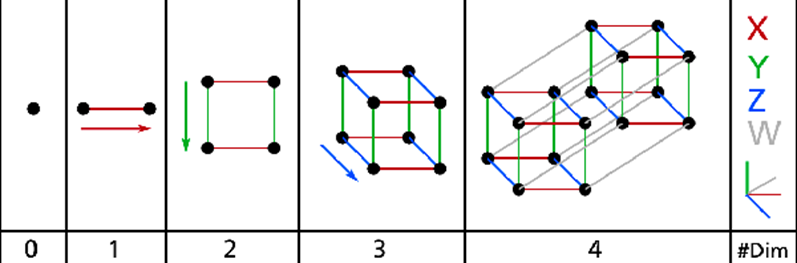
\includegraphics[height=0.7\textheight]{../machineLearningWeb/Figures/CH08/Hinh_8-1.png}\\
        \vspace{0.3cm}
        \textit{Hình 8-1. Điểm, đoạn thẳng, hình vuông, hình lập phương và tesseract (siêu hình lập phương từ 0D đến 4D)}
    \end{center}
\end{frame}

% Slide 8
\begin{frame}{Sự khác biệt khoảng cách trong không gian chiều cao}
    \begin{itemize}
        \item Nếu chọn hai điểm ngẫu nhiên trong một hình vuông 2D đơn vị, khoảng cách trung bình là $\approx 0.52$.
        \item Trong hình lập phương 3D đơn vị, khoảng cách trung bình là $\approx 0.66$.
        \item Trong một siêu hình lập phương đơn vị 1.000.000 chiều, khoảng cách trung bình là $\approx 408.25$.
        \item Có rất nhiều không gian trong các chiều cao, dẫn đến dữ liệu vô cùng thưa thớt (sparse).
    \end{itemize}
\end{frame}

% Slide 9
\begin{frame}{Nguy cơ quá khớp do thưa thớt}
    \begin{itemize}
        \item Tập dữ liệu có chiều cao $\rightarrow$ hầu hết các trường hợp huấn luyện cách rất xa nhau.
        \item Một trường hợp mới (test instance) có thể sẽ cách xa bất kỳ trường hợp huấn luyện nào đã biết.
        \item Dự đoán sẽ kém tin cậy hơn nhiều vì phải dựa trên các phép \textit{ngoại suy (extrapolation)} lớn.
        \item \textbf{Tóm lại:} Tập huấn luyện càng có nhiều chiều, nguy cơ \textbf{quá khớp (overfitting)} càng lớn.
    \end{itemize}
\end{frame}

% Slide 10
\begin{frame}{Các cách tiếp cận chính để giảm chiều}
    Thay vì cố gắng thu thập dữ liệu bằng số nguyên tử vũ trụ (để đủ độ dày đặc), chúng ta dùng các thuật toán giảm chiều:
    \begin{enumerate}
        \item \textbf{Phép chiếu (Projection)}
        \item \textbf{Học đa tạp (Manifold Learning)}
    \end{enumerate}
\end{frame}

% Slide 11
\begin{frame}{Cách tiếp cận 1: Phép chiếu (Projection)}
    \begin{itemize}
        \item Trong hầu hết các bài toán thực tế, các trường hợp huấn luyện không được phân bổ đều đặn (uniform) trên tất cả các chiều.
        \item Nhiều đặc trưng gần như không đổi, trong khi các đặc trưng khác tương quan mạnh.
        \item Kết quả là, mọi trường hợp huấn luyện thường nằm gọn trong (hoặc rất gần) một \textbf{không gian con (subspace) có số chiều thấp hơn nhiều} so với không gian gốc.
    \end{itemize}
\end{frame}

% Slide 12
\begin{frame}{Tập dữ liệu 3D gần không gian con 2D}
    \begin{center}
        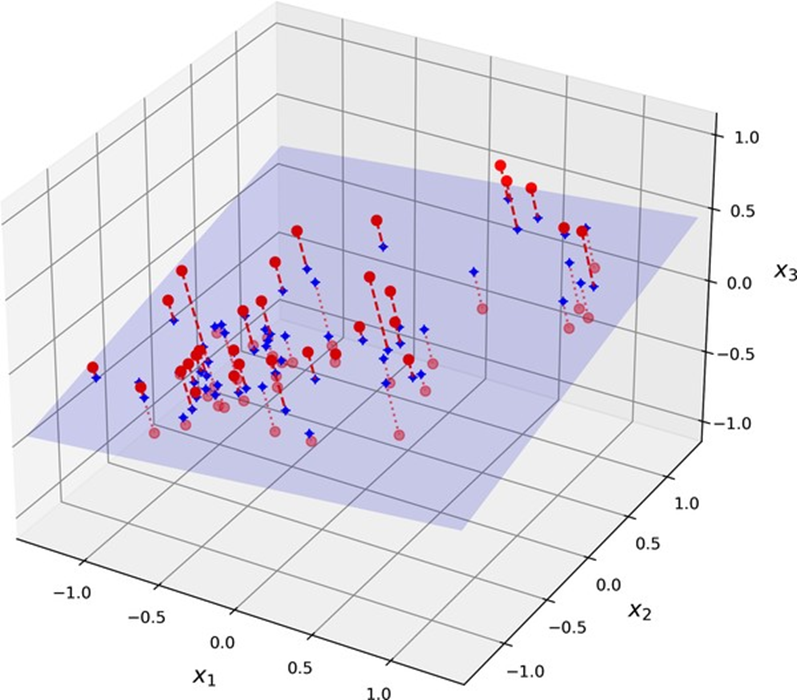
\includegraphics[height=0.7\textheight]{../machineLearningWeb/Figures/CH08/Hinh_8-2.png}\\
        \vspace{0.3cm}
        \textit{Hình 8-2. Một tập dữ liệu 3D nằm gần một không gian con 2D (mặt phẳng)}
    \end{center}
\end{frame}

% Slide 13
\begin{frame}{Tập dữ liệu 2D mới sau phép chiếu}
    \begin{center}
        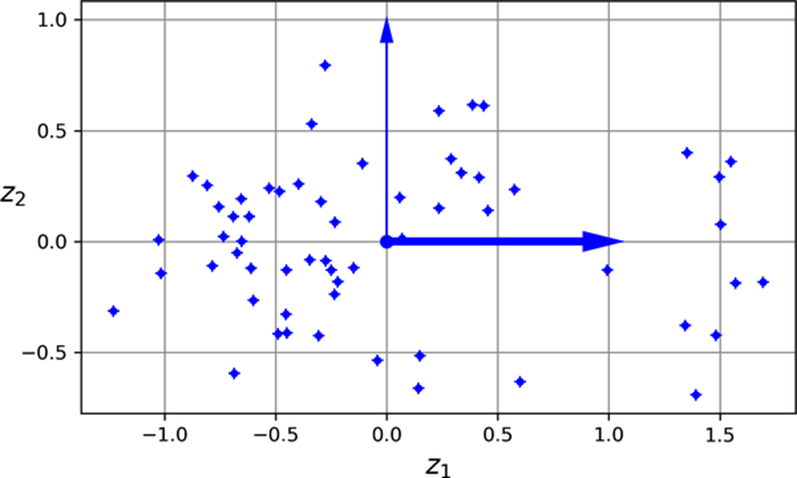
\includegraphics[height=0.7\textheight]{../machineLearningWeb/Figures/CH08/Hinh_8-3.png}\\
        \vspace{0.3cm}
        \textit{Hình 8-3. Bằng cách chiếu vuông góc các điểm lên mặt phẳng, ta thu được tập dữ liệu 2D mới}
    \end{center}
\end{frame}

% Slide 14
\begin{frame}{Cách tiếp cận 2: Học đa tạp (Manifold Learning)}
    \begin{itemize}
        \item Phép chiếu không phải lúc nào cũng là cách tiếp cận tốt nhất.
        \item Trong nhiều trường hợp, không gian con có thể bị \textbf{xoắn và uốn cong}.
        \item Ví dụ điển hình: Tập dữ liệu \textbf{Swiss roll}.
    \end{itemize}
\end{frame}

% Slide 15
\begin{frame}{Tập dữ liệu Swiss roll}
    \begin{center}
        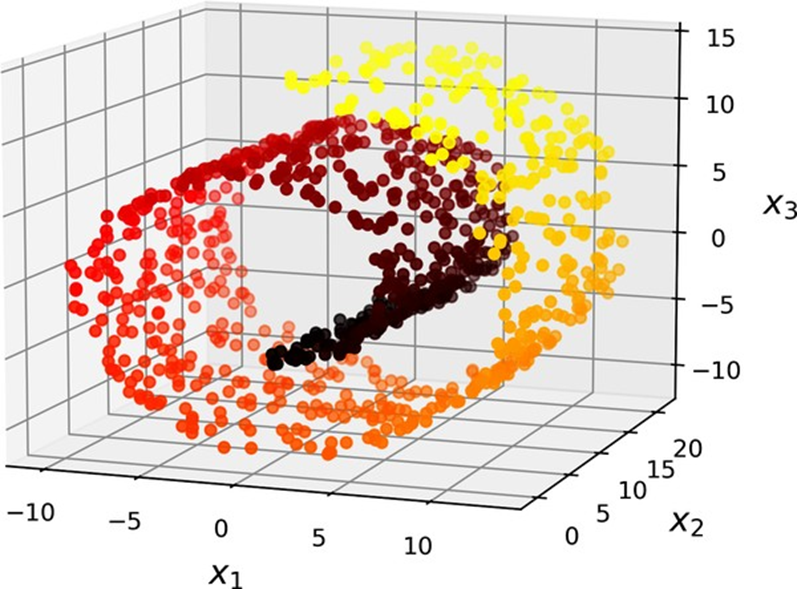
\includegraphics[height=0.7\textheight]{../machineLearningWeb/Figures/CH08/Hinh_8-4.png}\\
        \vspace{0.3cm}
        \textit{Hình 8-4. Tập dữ liệu Swiss roll (như một tờ giấy bị cuộn lại trong không gian 3D)}
    \end{center}
\end{frame}

% Slide 16
\begin{frame}{Làm dẹt (Phép chiếu) vs Mở cuộn (Đa tạp)}
    \begin{center}
        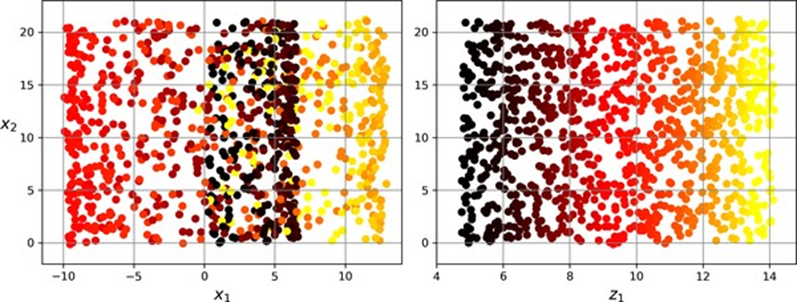
\includegraphics[width=0.9\textwidth]{../machineLearningWeb/Figures/CH08/Hinh_8-5.png}\\
        \vspace{0.3cm}
        \textit{Hình 8-5. Chiếu vuông góc làm dẹt cuộn (trái) - sai lầm; Mở cuộn (phải) - chính xác}
    \end{center}
\end{frame}

% Slide 17
\begin{frame}{Giả định đa tạp (Manifold Hypothesis)}
    \begin{itemize}
        \item \textbf{Đa tạp 2D:} là một hình 2D có thể bị uốn cong, xoắn lại trong một không gian có chiều cao hơn. Tổng quát, một đa tạp $d$-chiều nằm trong không gian $n$-chiều ($d<n$).
        \item \textbf{Giả định đa tạp:} Hầu hết các tập dữ liệu thực tế có chiều cao đều nằm gần một đa tạp có chiều thấp hơn nhiều.
        \item Các tác vụ học máy (như phân loại/hồi quy) \textbf{thường} sẽ đơn giản hơn nếu được biểu diễn trong không gian đa tạp (sau khi được mở cuộn).
    \end{itemize}
\end{frame}

% Slide 18
\begin{frame}{Lưu ý về Giả định đa tạp}
    \begin{center}
        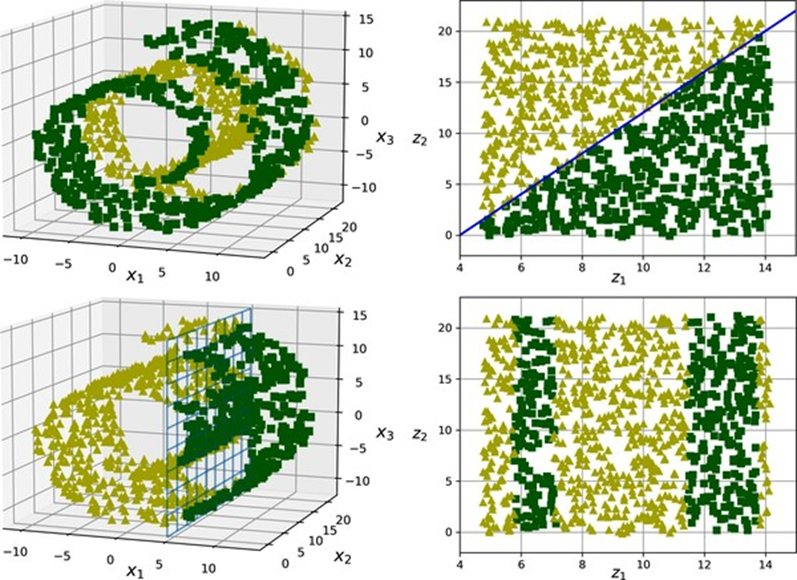
\includegraphics[height=0.65\textheight]{../machineLearningWeb/Figures/CH08/Hinh_8-6.png}\\
        \vspace{0.2cm}
        \textit{Hình 8-6. Đường biên quyết định không phải lúc nào cũng đơn giản hơn với không gian chiều thấp}
    \end{center}
\end{frame}

\section{Phân tích thành phần chính (PCA)}
% Slide 19
\begin{frame}{Phân tích thành phần chính (PCA)}
    \begin{itemize}
        \item \textbf{Phân tích thành phần chính (Principal Component Analysis - PCA)} cho đến nay là thuật toán giảm chiều phổ biến nhất.
        \item Nó là một phương pháp thuộc nhóm \textbf{Phép chiếu (Projection)}.
        \item Cơ chế: Đầu tiên xác định siêu phẳng (hyperplane) nằm gần dữ liệu nhất, sau đó chiếu toàn bộ dữ liệu lên mặt phẳng đó.
    \end{itemize}
\end{frame}

% Slide 20
\begin{frame}{Bảo toàn phương sai (Preserving Variance)}
    \begin{itemize}
        \item Trước khi chiếu dữ liệu, cần phải \textbf{chọn một siêu phẳng phù hợp}.
        \item PCA sẽ chọn siêu phẳng (hoặc trục) sao cho \textbf{bảo toàn được lượng phương sai lớn nhất} của dữ liệu.
        \item Việc này giúp giữ lại được nhiều thông tin nhất có thể sau phép chiếu.
        \item Nó cũng tương đương với việc chọn trục làm \textit{giảm thiểu khoảng cách bình phương trung bình} giữa tập dữ liệu gốc và điểm chiếu.
    \end{itemize}
\end{frame}

% Slide 21
\begin{frame}{Lựa chọn không gian con để chiếu}
    \begin{center}
        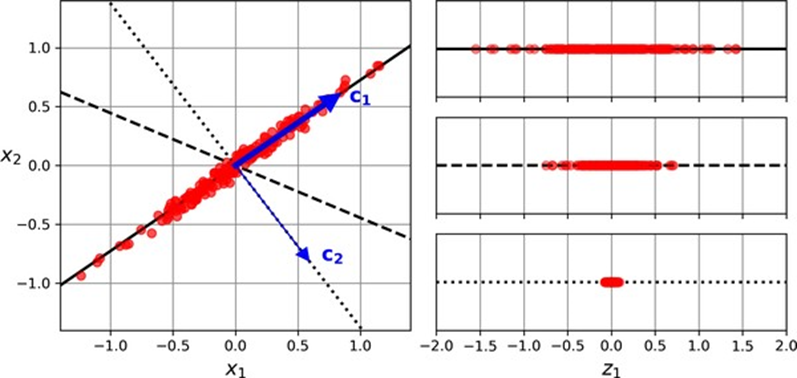
\includegraphics[height=0.7\textheight]{../machineLearningWeb/Figures/CH08/Hinh_8-7.png}\\
        \vspace{0.3cm}
        \textit{Hình 8-7. Phép chiếu lên đường liền nét bảo toàn phương sai tối đa}
    \end{center}
\end{frame}

% Slide 22
\begin{frame}{Các thành phần chính (Principal Components - PC)}
    \begin{itemize}
        \item PCA tìm trục có phương sai lớn nhất trong tập huấn luyện (Thành phần chính số 1 - PC1).
        \item Tiếp theo, nó tìm một trục thứ 2 \textbf{trực giao (vuông góc)} với trục 1 và chứa nhiều phương sai nhất từ phần còn lại (PC2).
        \item Quá trình tiếp diễn để tìm PC3, PC4... tối đa bằng số chiều của không gian gốc.
        \item Trục thứ $i$ được gọi là \textbf{thành phần chính thứ $i$} của dữ liệu.
    \end{itemize}
\end{frame}

% Slide 23
\begin{frame}{Toán học PCA: Phân tách giá trị số ít (SVD)}
    \begin{itemize}
        \item Để tìm tất cả các thành phần chính, ta sử dụng kỹ thuật phân tách ma trận tiêu chuẩn gọi là \textbf{Phân tách giá trị số ít (Singular Value Decomposition - SVD)}.
        \item SVD phân tách ma trận huấn luyện $X$ thành ba ma trận $U \cdot \Sigma \cdot V^T$.
        \item Ma trận $V^T$ chứa tất cả các thành phần chính cần tìm (các vector đơn vị trực giao).
        \item Công thức: $V^T = \begin{pmatrix} | & | & & | \\ c_1 & c_2 & \dots & c_n \\ | & | & & | \end{pmatrix}^T$
    \end{itemize}
\end{frame}

% Slide 24
\begin{frame}[fragile]{Tính toán PCA bằng NumPy (Phần 1)}
    Dùng hàm \texttt{svd()} của NumPy.
    \textbf{Lưu ý quan trọng:} PCA giả định rằng dữ liệu được \textit{căn giữa (centered)} xung quanh gốc tọa độ. Cần trừ đi trung bình trước khi chạy SVD.
    \begin{lstlisting}[language=Python]
import numpy as np

# Gia su X la tap du lieu cua ban
X_centered = X - X.mean(axis=0)

# Phan tach gia tri so it
U, s, Vt = np.linalg.svd(X_centered)

c1 = Vt[0] # Thanh phan chinh thu 1 (PC1)
c2 = Vt[1] # Thanh phan chinh thu 2 (PC2)
    \end{lstlisting}
\end{frame}

% Slide 25
\begin{frame}{Chiếu dữ liệu xuống d chiều}
    \begin{itemize}
        \item Sau khi có các thành phần chính (PC), ta có thể giảm kích thước không gian bằng cách chiếu tập dữ liệu lên siêu phẳng tạo bởi $d$ thành phần chính đầu tiên ($d < n$).
        \item Ma trận $W_d$ được định nghĩa là ma trận chứa $d$ cột đầu tiên của $V$ (hay $d$ hàng đầu tiên của $V^T$ chuyển vị).
        \item Phép chiếu: $X_{d-proj} = X \cdot W_d$
    \end{itemize}
\end{frame}

% Slide 26
\begin{frame}[fragile]{Thực hiện phép chiếu bằng NumPy}
    Đoạn mã sau chiếu tập huấn luyện lên mặt phẳng 2D định nghĩa bởi hai PC đầu tiên:
    \begin{lstlisting}[language=Python]
# Chon 2 thanh phan chinh dau tien va chuyen vi
W2 = Vt[:2].T

# Thuc hien phep nhan ma tran (phep chieu)
X2D = X_centered @ W2
    \end{lstlisting}
    Bây giờ \texttt{X2D} chính là dữ liệu 2D đã được giảm chiều, bảo toàn được tối đa lượng phương sai có thể từ tập $X$ ban đầu.
\end{frame}

% Slide 27
\begin{frame}[fragile]{Sử dụng Scikit-Learn cho PCA}
    Trong thực tế, Scikit-Learn cung cấp lớp \texttt{PCA} tự động xử lý SVD và quan trọng nhất là \textbf{tự động căn giữa dữ liệu}.
    \begin{lstlisting}[language=Python]
from sklearn.decomposition import PCA

pca = PCA(n_components=2)
X2D = pca.fit_transform(X)

# Lay cac vector thanh phan chinh
print(pca.components_)
    \end{lstlisting}
    \begin{itemize}
        \item \texttt{pca.components\_} chứa các thành phần chính đã tìm thấy.
    \end{itemize}
\end{frame}

% Slide 28
\begin{frame}{Tỷ lệ phương sai giải thích (Explained Variance Ratio)}
    \begin{itemize}
        \item Đây là một chỉ số quan trọng cho biết tỷ lệ phương sai của tập dữ liệu phân bổ dọc theo từng thành phần chính.
        \item Xem kết quả này qua biến \texttt{explained\_variance\_ratio\_}.
    \end{itemize}
\end{frame}

% Slide 29
\begin{frame}[fragile]{Đánh giá tỷ lệ phương sai giải thích}
    \begin{lstlisting}[language=Python]
>>> pca.explained_variance_ratio_
array([0.7578477 , 0.15186921])
    \end{lstlisting}
    \begin{itemize}
        \item Ý nghĩa: $\approx 76\%$ phương sai của dữ liệu nằm dọc theo trục PC1, và $\approx 15\%$ nằm trên trục PC2.
        \item Tổng cộng PC1 và PC2 giải thích được $>90\%$ phương sai. Điều này ngụ ý rằng các PC tiếp theo (PC3, PC4...) chứa rất ít thông tin hữu ích (chỉ còn khoảng $9\%$).
    \end{itemize}
\end{frame}

% Slide 30
\begin{frame}{Chọn số chiều phù hợp như thế nào?}
    \begin{itemize}
        \item \textbf{Quy tắc chung:} Trừ khi giảm xuống 2D hoặc 3D để vẽ biểu đồ trực quan, hãy chọn số chiều $d$ sao cho tổng phương sai được giữ lại đủ lớn (ví dụ: \textbf{95\%}).
        \item Nghĩa là, bạn sẽ thêm lần lượt PC1, PC2, PC3... cho đến khi tổng tỷ lệ phương sai giải thích vượt qua mức 95\%.
    \end{itemize}
\end{frame}

% Slide 31
\begin{frame}[fragile]{Tìm số chiều để giữ 95\% phương sai}
    Chạy PCA mà không giảm chiều để lấy toàn bộ các PCs, tính toán lũy kế:
    \begin{lstlisting}[language=Python]
from sklearn.datasets import fetch_openml
import numpy as np

mnist = fetch_openml('mnist_784', as_frame=False)
X_train = mnist.data[:60_000]

pca = PCA()
pca.fit(X_train)

cumsum = np.cumsum(pca.explained_variance_ratio_)
d = np.argmax(cumsum >= 0.95) + 1 
# d bang 154
    \end{lstlisting}
\end{frame}

% Slide 32
\begin{frame}[fragile]{Đặt n\_components là tỷ lệ phần trăm}
    Một cách tốt hơn (và nhàn hơn) là truyền thẳng mức độ phương sai bạn muốn bảo toàn dưới dạng một số thập phân từ 0.0 đến 1.0 cho \texttt{n\_components}:
    \begin{lstlisting}[language=Python]
# Scikit-learn se tu tinh toan so chieu toi thieu
pca = PCA(n_components=0.95)

X_reduced = pca.fit_transform(X_train)

print(pca.n_components_) 
# Output: 154
    \end{lstlisting}
\end{frame}

% Slide 33
\begin{frame}{Vẽ biểu đồ phương sai giải thích theo số chiều}
    Một phương pháp trực quan là vẽ mảng \texttt{cumsum} (phương sai tích lũy).
    \begin{center}
        (Giả lập Hình 8-8: Biểu đồ đường tăng dần và tạo thành một điểm uốn - elbow point - khi đạt $\approx 100-150$ chiều, sau đó đường đi ngang vì các chiều thêm vào không mang thêm phương sai.)
    \end{center}
    Tại "điểm uốn" (elbow), việc tăng thêm số chiều không mang lại quá nhiều giá trị thông tin, giúp người phân tích dễ dàng quyết định số chiều cần thiết.
\end{frame}

% Slide 34
\begin{frame}{Điều chỉnh số chiều như một siêu tham số}
    \begin{itemize}
        \item Nếu bạn sử dụng PCA như một bước \textit{tiền xử lý (preprocessing)} cho một tác vụ Machine Learning khác (ví dụ Rừng ngẫu nhiên), bạn có thể coi số chiều $d$ như một \textbf{siêu tham số (Hyperparameter)}.
        \item Có thể dùng \texttt{GridSearchCV} hoặc \texttt{RandomizedSearchCV} để tìm số chiều tốt nhất cho bài toán đó.
    \end{itemize}
\end{frame}

% Slide 35
\begin{frame}[fragile]{Sử dụng RandomizedSearchCV cho PCA}
    \begin{lstlisting}[language=Python]
from sklearn.ensemble import RandomForestClassifier
from sklearn.model_selection import RandomizedSearchCV
from sklearn.pipeline import make_pipeline

clf = make_pipeline(PCA(random_state=42), RandomForestClassifier(random_state=42))
param_distrib = {
    "pca__n_components": np.arange(10, 80),
    "randomforestclassifier__n_estimators": np.arange(50, 500)
}
rnd_search = RandomizedSearchCV(clf, param_distrib, n_iter=10, cv=3, random_state=42)
rnd_search.fit(X_train[:1000], y_train[:1000])

print(rnd_search.best_params_)
# pca__n_components toi uu chi la 23 thay vi 154
    \end{lstlisting}
\end{frame}

% Slide 36
\begin{frame}{PCA dùng để nén dữ liệu (Compression)}
    \begin{itemize}
        \item Sau khi áp dụng PCA bảo toàn 95\% phương sai, MNIST đã giảm từ 784 đặc trưng xuống còn 154.
        \item Tập dữ liệu lúc này chỉ còn bằng \textbf{$\approx 20\%$} kích thước ban đầu, trong khi chỉ \textbf{mất 5\% thông tin}!
        \item Mức độ nén tuyệt vời này giúp tiết kiệm bộ nhớ RAM và tăng tốc vượt trội thuật toán học máy phía sau.
    \end{itemize}
\end{frame}

% Slide 37
\begin{frame}{Tái tạo dữ liệu (Giải nén)}
    \begin{itemize}
        \item Bạn có thể \textit{giải nén} tập dữ liệu 154 chiều ngược trở lại thành 784 chiều.
        \item Tuy nhiên, đây là nén \textbf{có hao hụt (lossy compression)}, bạn sẽ không nhận lại được hoàn toàn 100\% pixel gốc (thiếu 5\% phương sai đã loại bỏ).
        \item Hình ảnh tái tạo sẽ bị mờ đi một chút, nhưng phần lớn nội dung gốc vẫn nguyên vẹn.
        \item \textit{Sai số tái tạo (Reconstruction Error):} Khoảng cách bình phương trung bình giữa dữ liệu gốc và dữ liệu giải nén.
    \end{itemize}
\end{frame}

% Slide 38
\begin{frame}[fragile]{Phép biến đổi ngược (inverse\_transform)}
    Sử dụng \texttt{inverse\_transform} trên đối tượng PCA:
    \begin{lstlisting}[language=Python]
X_recovered = pca.inverse_transform(X_reduced)
    \end{lstlisting}
    \begin{center}
        (Giả lập Hình 8-9: Hình ảnh MNIST gốc so sánh với hình ảnh đã qua nén/giải nén bằng PCA. Hình giải nén tuy không sắc nét hoàn hảo bằng nhưng vẫn dễ dàng đọc được là số mấy).
    \end{center}
\end{frame}

% Slide 39
\begin{frame}{PCA ngẫu nhiên (Randomized PCA)}
    \begin{itemize}
        \item Thuật toán \textbf{Randomized PCA} dùng kỹ thuật ngẫu nhiên hóa để xấp xỉ tìm $d$ thành phần chính đầu tiên một cách nhanh chóng.
        \item Độ phức tạp tính toán: $O(m \times d^2) + O(d^3)$, thay vì $O(m \times n^2) + O(n^3)$ của SVD tiêu chuẩn.
        \item Nó nhanh hơn đáng kể so với PCA đầy đủ khi $d \ll n$ (số chiều giảm xuống nhỏ hơn nhiều số chiều ban đầu).
    \end{itemize}
\end{frame}

% Slide 40
\begin{frame}[fragile]{Cài đặt Randomized PCA}
    Chỉ định tham số \texttt{svd\_solver="randomized"}:
    \begin{lstlisting}[language=Python]
rnd_pca = PCA(n_components=154, svd_solver="randomized", random_state=42)

X_reduced = rnd_pca.fit_transform(X_train)
    \end{lstlisting}
\end{frame}

% Slide 41
\begin{frame}{PCA tăng dần (Incremental PCA)}
    \begin{itemize}
        \item \textbf{Vấn đề của PCA thông thường:} Yêu cầu TOÀN BỘ tập dữ liệu phải nằm gọn trong bộ nhớ (RAM) cùng một lúc.
        \item \textbf{Giải pháp:} Incremental PCA (IPCA) cho phép bạn chia tập huấn luyện thành các \textit{mini-batch} và đẩy chúng vào mô hình từng lô nhỏ một.
        \item Hữu ích cho các tập dữ liệu khổng lồ (Out-of-core learning) và để áp dụng PCA theo thời gian thực (Online).
    \end{itemize}
\end{frame}

% Slide 42
\begin{frame}[fragile]{Cài đặt Incremental PCA với array\_split}
    Lưu ý gọi phương thức \texttt{partial\_fit()} ở từng bước thay vì \texttt{fit()}:
    \begin{lstlisting}[language=Python]
from sklearn.decomposition import IncrementalPCA
import numpy as np

n_batches = 100
inc_pca = IncrementalPCA(n_components=154)

for X_batch in np.array_split(X_train, n_batches):
    inc_pca.partial_fit(X_batch)

# transform ap dung cho toan bo
X_reduced = inc_pca.transform(X_train) 
    \end{lstlisting}
\end{frame}

% Slide 43
\begin{frame}[fragile]{Tối ưu Incremental PCA với tệp bộ nhớ (memmap)}
    Sử dụng \texttt{np.memmap} để sử dụng file nhị phân trên đĩa như thể nó nằm trong RAM. Dữ liệu chỉ tải vào RAM khi cần:
    \begin{lstlisting}[language=Python]
# doc file da luu duoi dang memmap
filename = "my_mnist.mmap"
X_mmap = np.memmap(filename, dtype="float32", mode="readonly").reshape(-1, 784)

batch_size = X_mmap.shape[0] // n_batches
inc_pca = IncrementalPCA(n_components=154, batch_size=batch_size)

# inc_pca hieu cach hoat dong cua memmap va se lay tung doan du lieu theo batch_size
inc_pca.fit(X_mmap)
    \end{lstlisting}
\end{frame}

\section{Phép chiếu ngẫu nhiên \& LLE}
% Slide 44
\begin{frame}{Phép chiếu ngẫu nhiên (Random Projection)}
    \begin{itemize}
        \item Chiếu dữ liệu xuống không gian thấp bằng một \textbf{ma trận ngẫu nhiên}.
        \item Thay vì dùng SVD phức tạp, Random Projection chứng minh rằng một ma trận chiếu tạo ngẫu nhiên \textit{rất có khả năng bảo toàn khoảng cách} giữa các điểm dữ liệu.
        \item Ưu điểm: \textbf{Không cần huấn luyện!} Chỉ phụ thuộc vào hình dạng ma trận ban đầu. Rất nhẹ và cực nhanh cho dữ liệu chiều cực lớn (hàng chục nghìn features).
    \end{itemize}
\end{frame}

% Slide 45
\begin{frame}{Định lý Johnson-Lindenstrauss}
    \begin{itemize}
        \item \textbf{Định lý Johnson-Lindenstrauss (JL):} Có thể chiếu $m$ điểm từ không gian chiều cao xuống không gian $d$ chiều sao cho khoảng cách bình phương giữa mọi cặp điểm chỉ bị méo mó tối đa là một sai số $\varepsilon$.
        \item Ví dụ: Bạn có 5.000 điểm ($m$), với dung sai $\varepsilon=0.1$.
        \item Định lý tính được $d \approx 7300$ chiều là đủ an toàn. Phương trình này \textbf{không quan tâm đến số chiều gốc} $n$ (ngay cả khi $n = 1$ triệu).
    \end{itemize}
\end{frame}

% Slide 46
\begin{frame}[fragile]{Tìm số chiều tối thiểu bảo toàn khoảng cách}
    Sử dụng Scikit-Learn để tính toán theo JL lemma:
    \begin{lstlisting}[language=Python]
from sklearn.random_projection import johnson_lindenstrauss_min_dim

m = 5000  # so truong hop
eps = 0.1 # dung sai

d = johnson_lindenstrauss_min_dim(m, eps=eps)
print(d) 
# Output: 7300
    \end{lstlisting}
\end{frame}

% Slide 47
\begin{frame}[fragile]{Phép chiếu ngẫu nhiên thủ công}
    Tạo một ma trận $P$ lấy mẫu từ phân phối chuẩn và nhân trực tiếp:
    \begin{lstlisting}[language=Python]
import numpy as np

n = 20_000 # so chieu ban dau
m = 5_000  # so mau
d = 7300   # chieu muc tieu

# Tao ma tran ngau nhien P
P = np.random.randn(d, n) / np.sqrt(d)

X = np.random.randn(m, n) 

# Thuc hien giam chieu
X_reduced = X @ P.T 
    \end{lstlisting}
\end{frame}

% Slide 48
\begin{frame}[fragile]{Scikit-Learn Random Projections}
    Dễ dàng hơn với 2 lớp xây dựng sẵn:
    \begin{lstlisting}[language=Python]
from sklearn.random_projection import GaussianRandomProjection
from sklearn.random_projection import SparseRandomProjection

# 1. Gaussian Random Projection
gaussian_rnd_proj = GaussianRandomProjection(eps=0.1, random_state=42)
X_reduced = gaussian_rnd_proj.fit_transform(X)

# 2. Sparse Random Projection
sparse_rnd_proj = SparseRandomProjection(eps=0.1)
# Hoat dong tuong tu nhung ma tran chieu hinh thanh chu yeu bang so 0.
# Giup tiet kiem RAM cuc manh (vd 25MB thay vi 1.2GB)
    \end{lstlisting}
\end{frame}

% Slide 49
\begin{frame}{Nhúng tuyến tính cục bộ (Locally Linear Embedding - LLE)}
    \begin{itemize}
        \item Là một kỹ thuật \textbf{Giảm chiều phi tuyến tính (NLDR)} và thuộc họ \textbf{Học đa tạp (Manifold Learning)}.
        \item Không sử dụng phép chiếu như PCA. 
        \item \textbf{Cơ chế:} 
        \begin{enumerate}
            \item Đo lường cách mỗi điểm liên kết tuyến tính với các điểm láng giềng gần nhất của nó.
            \item Tìm biểu diễn chiều thấp sao cho mối liên kết (khoảng cách cục bộ) này được \textbf{bảo toàn tốt nhất}.
        \end{enumerate}
        \item Tuyệt vời để mở cuộn các đa tạp bị xoắn (như Swiss roll) nếu dữ liệu không có quá nhiều nhiễu.
    \end{itemize}
\end{frame}

% Slide 50
\begin{frame}[fragile]{Sử dụng LocallyLinearEmbedding cho Swiss roll}
    \begin{lstlisting}[language=Python]
from sklearn.datasets import make_swiss_roll
from sklearn.manifold import LocallyLinearEmbedding

# Tao du lieu Swiss roll 3D
X_swiss, t = make_swiss_roll(n_samples=1000, noise=0.2, random_state=42)

# Giam xuong 2D bang LLE, danh gia tren 10 lang gieng gan nhat
lle = LocallyLinearEmbedding(n_components=2, n_neighbors=10, random_state=42)
X_unrolled = lle.fit_transform(X_swiss)
    \end{lstlisting}
    \begin{center}
        (Giả lập Hình 8-10: Dữ liệu Swiss Roll 3D được "mở cuộn" thành một mặt phẳng 2D thành công, duy trì quan hệ giữa các điểm bên cạnh nhau).
    \end{center}
\end{frame}

% Slide 51
\begin{frame}{Thuật toán LLE: Bước 1 (Mô hình hóa cục bộ)}
    \begin{itemize}
        \item Đối với mỗi điểm $x^{(i)}$, LLE tìm $k$ láng giềng gần nhất của nó.
        \item Sau đó cố gắng \textbf{tái tạo điểm $x^{(i)}$} như một hàm tuyến tính (tổng có trọng số) của $k$ láng giềng đó.
        \item Mục tiêu: Tìm các trọng số $w_{i,j}$ sao cho khoảng cách bình phương giữa $x^{(i)}$ và $\sum w_{i,j}x^{(j)}$ là nhỏ nhất có thể.
        \item Kết thúc bước 1, ta có một ma trận trọng số $W$ phản ánh chính xác cấu trúc hình học \textbf{cục bộ} của tập dữ liệu trong không gian gốc (chiều cao).
    \end{itemize}
\end{frame}

% Slide 52
\begin{frame}{Thuật toán LLE: Bước 2 (Giảm chiều bảo toàn khoảng cách)}
    \begin{itemize}
        \item Ánh xạ các điểm vào không gian $d$ chiều (với $d < n$).
        \item Giữ nguyên ma trận trọng số $W$ đã tìm ở Bước 1.
        \item Tìm các vị trí điểm mới (tọa độ mới) trong không gian $d$ chiều, sao cho chúng \textbf{vẫn thỏa mãn ma trận trọng số} đó càng gần càng tốt.
        \item \textit{Điểm yếu của LLE:} Mở rộng kém cho tập dữ liệu rất lớn.
    \end{itemize}
\end{frame}

% Slide 53
\begin{frame}{Các kỹ thuật giảm chiều khác: MDS \& Isomap}
    \begin{itemize}
        \item \textbf{MDS (Multidimensional Scaling):} Cố gắng giảm chiều trong khi bảo toàn \textbf{khoảng cách vật lý} giữa các trường hợp như ở không gian gốc. Làm phẳng thay vì mở cuộn.
        \item \textbf{Isomap:} Xây dựng đồ thị nối các láng giềng, sau đó giảm chiều trong khi bảo toàn \textbf{khoảng cách trắc địa (geodesic distance)} giữa các điểm. (Trắc địa là đi qua các điểm kết nối, không phải bay đường chim bay). Thích hợp mở cuộn đa tạp.
    \end{itemize}
\end{frame}

% Slide 54
\begin{frame}{Các kỹ thuật giảm chiều khác: t-SNE \& LDA}
    \begin{itemize}
        \item \textbf{t-SNE (t-Distributed Stochastic Neighbor Embedding):} Giảm chiều bằng cách giữ các điểm tương đồng ở gần nhau, nhưng đẩy các điểm dị biệt ra thật xa. Đặc biệt tốt để \textbf{phát hiện cụm trực quan} (như vẽ bản đồ MNIST 2D).
        \item \textbf{LDA (Linear Discriminant Analysis):} Một thuật toán \textbf{Phân loại} (Classification). Trong quá trình huấn luyện nó sẽ học trục phân biệt rõ rệt nhất giữa các lớp. Bạn dùng trục này để chiếu dữ liệu, giúp giữ cho các nhãn cách xa nhau nhất có thể $\rightarrow$ Tiền xử lý tuyệt vời cho thuật toán phân loại khác.
    \end{itemize}
\end{frame}

% Slide 55
\begin{frame}{Tổng kết Chương 8}
    \begin{itemize}
        \item \textbf{Khái niệm \& Động lực:} Giảm số chiều dữ liệu giúp phòng tránh "Lời nguyền số chiều", tăng tốc mô hình và khả năng trực quan hóa.
        \item \textbf{PCA:} Phương pháp Phép chiếu, sử dụng SVD, là kỹ thuật mặc định ưu tiên số một. Nắm vững Incremental PCA (cho dữ liệu lớn) và Randomized PCA.
        \item \textbf{Random Projection:} Vô địch về tốc độ và tiết kiệm RAM cho dữ liệu siêu lớn mà không cần huấn luyện.
        \item \textbf{Manifold Learning (LLE, Isomap...):} Có khả năng "mở cuộn" các hình khối xoắn ốc phức tạp, thích hợp cho dữ liệu có cấu trúc đa tạp phi tuyến tính.
    \end{itemize}
\end{frame}

% Slide 56
\begin{frame}{Hỏi \& Đáp}
    \begin{center}
        \Large{\textbf{CẢM ƠN CÁC BẠN ĐÃ LẮNG NGHE!}}\\
        \vspace{1cm}
        Q \& A
    \end{center}
\end{frame}

\end{document}
